\documentclass[turkish,12pt,red,compress,mathserif]{beamer}
\usepackage[utf8]{inputenc}
\usepackage{verbatim}
\usepackage{listings}
\usepackage{url}

\usetheme{Warsaw}
\setbeamertemplate{navigation symbols}{}
\setbeamertemplate{footline}[page number]
\lstset{basicstyle=\tiny,showstringspaces=false}

\title{A Generic C/C++ API \\
  for Wireless Interfaces \\
  in GNU/Linux Systems}
\author{Volkan Yazıcı \\
  Özyeğin University \\
  Dept. of Electrical \& Electronics Engineering \\
  \emph{volkan.yazici@ozyegin.edu.tr}}

\date[Fall 2010]{WISERLAB Group Meeting, İstanbul, 2010}

\begin{document}

\begin{frame}\titlepage\end{frame}
\begin{frame}\tableofcontents\end{frame}

%%%%%%%%%%%%%%%%%%%%%%%%%%%%%%%%%%%%%%%%%%%%%%%%%%%%%%%%%%%%%%%%%%%%%%%%%%%%%%%%

\section{Intro.}

%-------------------------------------------------------------------------------

\subsection{Motivation}

\begin{frame}{Motivation}
  \begin{itemize}
  \item A generic C/C++ API for network interfaces.
    \begin{itemize}
    \item Almost full coverage of wireless network configurations.
      \begin{itemize}
      \item \texttt{iwconfig}
      \item \texttt{iwlist}
      \item \texttt{wlanconfig}
      \end{itemize}
    \item Generic network interface operations.
      \begin{itemize}
      \item \texttt{ifconfig}
      \item \texttt{route}
      \end{itemize}
    \end{itemize}
  \item A \alert{library}, not a command line tool.
  \item A core component of the \alert{Connectivity Brokerage}.
  \end{itemize}
\end{frame}

%-------------------------------------------------------------------------------

\subsection{Literature}

\begin{frame}{Literature}
  \begin{itemize}
  \item A majority of the previous works were basically parsing command (e.g.
    \texttt{iwlist}) outputs.
  \item Accessing command line tools within a program execution flow is
    dangerous and not convenient.
    \begin{itemize}
    \item Command outputs are unreliable.
      \begin{itemize}
      \item High possibility of unknown outputs (bugs).
      \item Hard to be in sync. with every release.
      \item Requires a significant amount of work to parse and extract certain
        tokens.
      \end{itemize}
    \end{itemize}
  \end{itemize}
\end{frame}

\begin{frame}{Literature (Cont'd)}
  \begin{itemize}
  \item Other libraries with similar goals:
    \begin{itemize}
    \item \texttt{libiw} of Wireless Tools for Linux,
    \item \texttt{libnm} of NetworkManager.
    \end{itemize}
  \item Cons:
    \begin{itemize}
    \item not designed for embedded environments (library dependencies),
    \item function calls are blocking,
    \item lacks ifup/ifdown and routing table functionalities,
    \item no fine-grained access to the configurations,
    \item doesn't provide an easy to use unified API.
    \end{itemize}
  \end{itemize}
\end{frame}

%%%%%%%%%%%%%%%%%%%%%%%%%%%%%%%%%%%%%%%%%%%%%%%%%%%%%%%%%%%%%%%%%%%%%%%%%%%%%%%%

\section{Contrib.}

\begin{frame}{Contribution}
  \begin{itemize}
  \item a \textbf{unified C/C++ library} with on par features compared to
    \texttt{iwconfig}, \texttt{iwlist}, \texttt{wlanconfig}, \texttt{ifconfig},
    \texttt{route} tools.
  \item not yet another command wrapper, but a written from scratch library
    accessing network drivers through \textbf{\texttt{ioctl()} calls to the
      kernel} and \textbf{nl80211} netlink.
  \item \textbf{fine-grained access}, that is, just get/set a single property at
    a time.
  \item \textbf{non-blocking function calls}.
  \item code base is not bloated with 10 year old backward compatibility issues.
  \item fully \textbf{documented, clean code}; suitable for research \&
    education purposes.
  \end{itemize}
\end{frame}

%%%%%%%%%%%%%%%%%%%%%%%%%%%%%%%%%%%%%%%%%%%%%%%%%%%%%%%%%%%%%%%%%%%%%%%%%%%%%%%%

\section{Status}

\subsection{Where Are We?}

\begin{frame}{Where Are We?}
  \begin{itemize}
  \item \textbf{Finished!} (Yeah we did!)
    \begin{itemize}
    \item Website \& Docs.: \url{http://vy.github.com/wapi/}
    \item Source Code: \url{http://www.github.com/vy/wapi/}
    \end{itemize}
  \item Tested on various hardware. (Atheros, Broadcom, etc.)
  \item Fully documented code base. (Thanks Doxygen.)
  \item Now available as an \textbf{official OpenWrt package}!
  \end{itemize}
\end{frame}

%-------------------------------------------------------------------------------

\subsection{Roadmap}

\begin{frame}{Roadmap}
  \begin{itemize}
  \item Get rid off \texttt{libiw} dependency.
    \begin{itemize}
    \item Because of a race-condition bug in \texttt{nl80211}, delayed for a
      while.
    \end{itemize}
  \end{itemize}
\end{frame}


%%%%%%%%%%%%%%%%%%%%%%%%%%%%%%%%%%%%%%%%%%%%%%%%%%%%%%%%%%%%%%%%%%%%%%%%%%%%%%%%

\section{Demo}

%-------------------------------------------------------------------------------

\subsection{Getters}

\begin{frame}[fragile]{Getters: Source Code}
  \begin{lstlisting}[language=c]
int ret;
double freq;
wapi_freq_flag_t freq_flag;
char essid[WAPI_ESSID_MAX_SIZE + 1];
wapi_essid_flag_t essid_flag;

...

/* freq */
ret = wapi_get_freq(sock, ifname, &freq, &freq_flag);
printf("freq: %g\n", freq);
printf("freq_flags: %s\n", wapi_freq_flags[freq_flag]);

/* essid */
ret = wapi_get_essid(sock, ifname, essid, &essid_flag);
printf("essid: %s\n", essid);
printf("essid_flag: %s\n", wapi_essid_flags[essid_flag]);

...
  \end{lstlisting}
\end{frame}

\begin{frame}[fragile]{Getters: Output}
  \begin{lstlisting}
ip: 192.168.1.111
netmask: 255.255.255.0
freq: 2.412e+09
freq_flag: WAPI_FREQ_AUTO
chan: 1
freq: 2.412e+09
essid: ozu
essid_flag: WAPI_ESSID_ON
mode: WAPI_MODE_MANAGED
ap: 00:14:C1:34:CE:83
wireless.c:451:wapi_get_bitrate(): Bitrate is disabled.
wireless.c:546:wapi_get_txpower():ioctl(SIOCGIWTXPOW): Invalid argument
  \end{lstlisting}
\end{frame}

%-------------------------------------------------------------------------------

\subsection{Scanning}

\begin{frame}[fragile]{Scanning: Source Code}
  \begin{lstlisting}[language=c]
int sleepdur = 1;
int sleeptries = 5;
wapi_list_t list;
wapi_scan_info_t *info;
int ret;

/* start scan */
ret = wapi_scan_init(sock, ifname);
printf("wapi_scan_init(): ret: %d\n", ret);

/* wait for completion */
do {
    sleep(sleepdur);
    ret = wapi_scan_stat(sock, ifname);
    printf("wapi_scan_stat(): ret: %d, sleeptries: %d\n", ret, sleeptries);
} while (--sleeptries > 0 && ret > 0);
if (ret < 0) return;

/* collect results */
bzero(&list, sizeof(wapi_list_t));
ret = wapi_scan_coll(sock, ifname, &list);
printf("wapi_scan_coll(): ret: %d\n", ret);

/* print found aps */
for (info = list.head.scan; info; info = info->next)
    printf(">> @%xl %s\n", (size_t) info, (info->has_essid ? info->essid : ""));
  \end{lstlisting}
\end{frame}

\begin{frame}[fragile]{Scanning: Output}
  \begin{lstlisting}
wapi_scan_init(): ret: 0
wapi_scan_stat(): ret: 1, sleeptries: 5
wapi_scan_stat(): ret: 0, sleeptries: 4
wapi_scan_coll(): ret: 0
>> @8214ce8l OzuNet.Visitors
>> @8214c90l Wozunacad
>> @8214c38l OzuNet.Visitors
>> @8214be0l canbazoglu
>> @8214b88l NWii
>> @8214b30l wozunguest
>> @8214ad8l Wozunacad
>> @8214a80l ZQNET29
>> @8214a28l wozunvisitor
>> ...
  \end{lstlisting}
\end{frame}

%%%%%%%%%%%%%%%%%%%%%%%%%%%%%%%%%%%%%%%%%%%%%%%%%%%%%%%%%%%%%%%%%%%%%%%%%%%%%%%%

\section{Doc.}

\begin{frame}{Doxygen}
  \begin{itemize}
  \item All available public API (functions, variables, constants, structs,
    enums, etc.) is fully documented.
  \item Driver specific turnarounds are documented.
  \item All documentation is integrated within the source code itself as comment
    lines.
  \item Using Doxygen to produce HTML, LaTeX, RTF, etc. output from these
    comment lines.
  \end{itemize}
\end{frame}

\begin{frame}
  \centering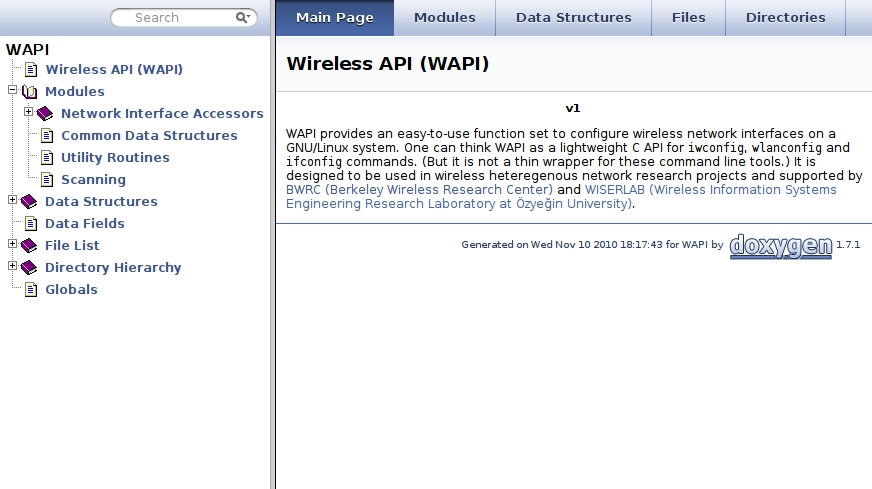
\includegraphics[width=\textwidth]{dox1.jpg}
\end{frame}

\begin{frame}
  \centering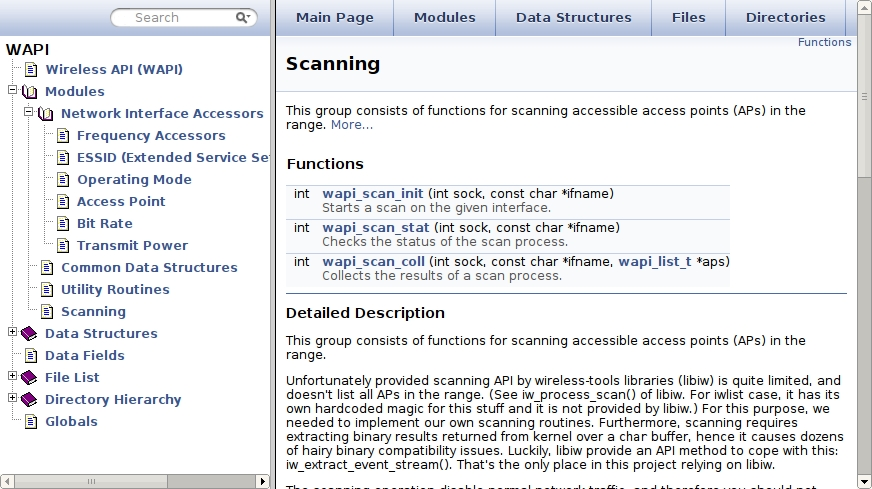
\includegraphics[width=\textwidth]{dox2.jpg}
\end{frame}

\begin{frame}
  \centering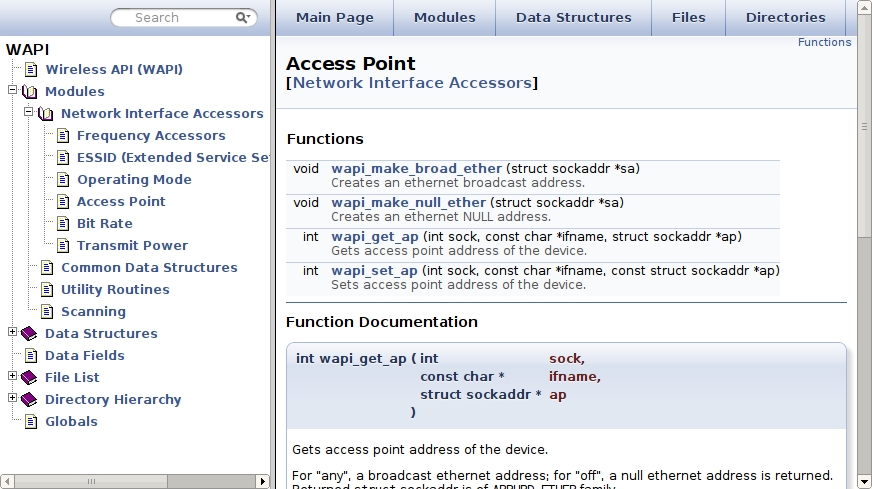
\includegraphics[width=\textwidth]{dox3.jpg}
\end{frame}

\begin{frame}
  \centering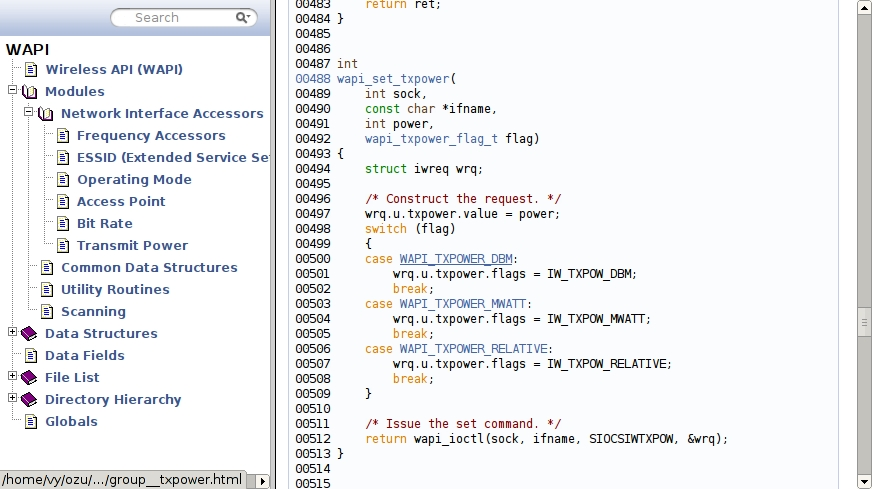
\includegraphics[width=\textwidth]{dox4.jpg}
\end{frame}

%%%%%%%%%%%%%%%%%%%%%%%%%%%%%%%%%%%%%%%%%%%%%%%%%%%%%%%%%%%%%%%%%%%%%%%%%%%%%%%%

\section{Questions}

\begin{frame}{Questions?}
  \begin{figure}
    \centering
\includegraphics{feeling-lucky.jpg}
  \end{figure}
\end{frame}

%%%%%%%%%%%%%%%%%%%%%%%%%%%%%%%%%%%%%%%%%%%%%%%%%%%%%%%%%%%%%%%%%%%%%%%%%%%%%%%

\end{document}
